\section{Continuous Query-Based Syndication}

Continuous Query-Based Syndication (CQBS) is a hybrid publish-subscribe pattern that provides the expressiveness of content-based systems while retaining the simplicity of topic-based systems.
The goal of CQBS is to provide a messaging system that can account for and adapt to the heterogeneity of data sources in the IoT.
CQBS allows embedded publishers to describe themselves using rich metadata, and provides subscribers with the ability to discover and subscribe to relevant data sources and maintain a consistent view of the context of those sources.

Here, we first establish the CQBS primitives---streams and metadata---before delving into how CQBS operates and what roles publishers and subscribers play.
We then describe the design and implementation of an individual broker (we defer the discussion of the full distributed system to Section~\ref{section:coordinator}).

\begin{figure}
\centering
\begin{lstlisting}[language=pseudocode,basicstyle=\small]
UUID = "dd9ef92e-140a-11e6-b352-1002b58053c7"
# register client
metadata = {
  UUID = UUID,
  Location/Room = "410",
  Location/Building = "Soda",
  Location/City = "Berkeley",
  Point/Type = "Sensor",
  Point/Measure = "Temperature"
  UnitofMeasure = "Fahrenheit",
  UnitofTime = "ms",
  Timezone = "America/Los_Angeles"
}
register_msg := msgpack.encode(metadata)
send_to_broker(register_msg)
while True:
    temp_val := read_sensor()
    msg := msgpack.encode({
            UUID = UUID,
            Value = temp_val
           })
    send_to_broker(msg)
    sleep(10)
\end{lstlisting}
\caption{Client registration and publishing pseudocode}
\label{fig:pseudoclient}
\end{figure}

\subsection{Streams and Metadata}

A stream is a virtual representation of a specific sensor or actuator channel (a ``capability'') that is indexed by a 16-byte universally unique identifier (UUID).
Each stream is described by \emph{metadata}, which is a bag of key-value pairs: keys are required to be strings, but values may be any one-dimensional data type\footnote{In our implementation, values are restricted to strings: see Section~\ref{section:evaluation}.}.
Key-value pairs are most effective when drawn from some well-known ontology (such as Semantic Sensor Web~\cite{sheth2008semantic}), but our system places no restrictions on their content.
The association of metadata to a stream is done by the UUID; when a publisher creates a new stream, it registers that stream with the broker by sending a message containing the UUID and all of the metadata.
The broker (or the coordinator, in the distributed case) stores the mapping from stream UUID to metadata.
A publisher changes metadata by sending the ``diff'' of which keys and values have changed.
A given producer (data provider) can have as many streams as it wishes.
Each message contains at least the UUID of the originating stream, and can also contain any metadata changes, and of couse the published value itself, which can be any serializable object.

An example of metadata for a temperature sensor, and the basic client logic, can be found in Figure~\ref{fig:pseudoclient}.
In the initial registration message, along with the other metadata, the reporting process describes the thermostat as being in room 410 Soda.
If this changes, such as if the sensor were on a piece of smart clothing or furniture, the sensor attaches the metadata update \lstinline[language=SQL,basicstyle=\ttfamily]{Location/Room = "415"} to any outgoing message, where it is handled by the broker (described in the following section).
A discussion of client complexity can be found in Section~\ref{section:evaluation}.

This is a departure from the approach of content-based pub-sub systems, where although the producer may possess some unique identifier, it transmits any associated ``content'' (metadata) in every message.
This verbose design choice may be appropriate for distributed sytems in which a publisher is a larger application that produces many different types of data, but when the data per-producer is relatively static (temperature sensors will always report temperature data), this flexibility is unneeded.
It becomes more efficient to essentially ``cache'' the metadata of a publisher in a central location where it can be used for syndication.

The simple structure of a stream (essentially a set of special key-value pairs) means a stream can be well represented in nearly any application protocol.
We choose MsgPack, a lean, typed binary serialization format that is simple enough to be encoded/decoded on embedded devices with limited code space.

%\subsection{Clients}

%Clients are distributed, continuously running processes that are producers and consumers of streams and updates to metadata.
%The streams produced by clients represent the set of sensors, actuators and capabilities available to be discovered, consumed and used.

% \emph{message} is the unit of communication in all interactions between
%clients and the broker. Messages sent from clients are either a query string
%for initiating a subscription or one-off response, or a structured packet
%containing the UUID of some stream and optionally an array of readings and/or a
%set of metadata updates. Examples of when metadata updates occur include when a
%device is registered (i.e.  sending the initial configuration), when a device
%changes location, or when a equipment attached to a device is changed such as
%installing an occupancy-driven switch for a lighting system.  Messages sent by
%the broker consist of forwarded client messages and ``diffs'' that convey
%changes in the set of streams matching a client's query.
%Figure~\ref{fig:messages} contains an example exchange of messages for
%a continuous query.
%
%Upon startup, a client registers streams it produces by sending messages
%containing metadata describing each one (see Figure~\ref{fig:message}). This makes
%the stream discoverable by and visible to other clients. Reporting data is
%straightforward: clients simply send messages with a stream's identifier and
%latest timestamped readings to the broker (the \texttt{UUID} and
%\texttt{Readings} fields). The broker forwards these readings to any subscribed
%clients as it receives them.
%
%In addition to producing streams, clients can also consume streams by
%expressing subscriptions to the broker in the form of SQL-like queries (see
%Section~\ref{section:syndication}). These queries are how clients perform
%discovery, receive timeseries data, and receive actuation requests.
%In dynamic environments typical of the Internet of Things, the results of
%these queries can become stale if they are executed only once. The broker
%continuously evaluates these queries to provide clients with a consistent view
%of their operating context.
%
%\subsection{Giles Architecture} \label{subsection:architecture}
%
%In this section, we present an overview of the six components of
%the Giles architecture.  These components handle incoming messages and queries
%for archival and delivery, and maintain consistent routes for query-based
%syndication.  This architecture is illustrated in
%Figure~\ref{fig:architecture}.
%
%\textbf{Protocol Plugin}: Protocol plugins do the work of translating messages
%between an application protocol and canonical message form. For
%simple request-response cases, the plugin translates the request, relays
%the message to the Giles API, then converts the result back to the original
%application protocol format and responds to the client. For the streaming
%functionality required by query-based syndication, the plugin maintains the
%connection to each client, and provides a handler to the Giles API that is
%called whenever an event is to be sent to an associated client.
%
%\textbf{API}: protocol plugins interface express how an incoming
%message should be interpreted. In terms of incoming data, Giles only deals with
%queries and messages (updates on streams involving metadata and/or new
%timeseries data), but can process them differently depending on the context.
%The API hands the incoming data to the correct pipeline.
%
%
%\textbf{Authorization Manager}: Giles enforces read/write permissions on a
%stream by stream basis. Considering the large numbers of devices and contexts
%predicted in the Internet of Things, it is important that
%administration of the system needs to scale, not just the system itself. Giles
%uses group-based permissions, rather than individual permissions, to avoid
%micromanagement of permissions surrounding increasing numbers of applications and users. All individual
%interactions with Giles carry an \emph{ephemeral key} which has an expiry and
%can be revoked; this key maps onto a set of roles. For each incoming
%interaction, the authorization manager does the work of evaluating the key's
%associated roles with the streams involved in the interaction, and adjusts the
%result set appropriately.
%
%\textbf{Broker}: While protocol plugins handle the network element of
%publishing and subscribing, the broker component provides routing
%between publishers and subscribers. This is done by maintaining mappings between clients, their associated
%queries, and the streams associated with those queries. These mappings are kept
%consistent in-band with the rest of the system, as discussed in
%Section~\ref{subsection:eventdriven} and seen in Figure~\ref{fig:evaluatequery}.
%
%\textbf{Query Processor}: The query processor parses all incoming queries and
%uses the outputted abstract syntax tree (AST) to adjust broker data structures
%(detailed in Figure~\ref{fig:evaluatequery}). This component also handles
%communication to and from the metadata and timeseries databases, and
%reevaluates subscription queries on behalf of the broker.
%
%\textbf{Timeseries Database}: Giles' role as a broker makes it a logical
%location to do archival of incoming data. Even in a distributed setting with
%multiple broker instances, Giles' visibility into all routed data means that
%archival can be performed without explicit action by clients. This is in
%contrast to other service composition systems (e.g. AllJoyn~\cite{alljoyn},
%SDS~\cite{czerwinski1999architecture},
%Jini~\cite{gupta2002jini}\cite{rigole2002using}\cite{waldo1999jini}) that
%perform archival as a secondary feature. All participants in such a system must
%duplicate all data to be archived and communicate that directly with an
%archival service. In Giles, all data and interactions are archived
%automatically and can be queried. Giles stores timeseries data in a dedicated
%timeseries store that is updated dynamically as clients report.
%
%\textbf{Metadata Database}: The Giles metadata model is simple enough to not
%place unusual requirements on the choice of a backend database.  Streams are
%wholly defined by their UUID and metadata, so the database only needs to store
%associations of UUID to metadata, and provide query facilities for retrieving
%metadata for a given UUID and retrieving all UUIDs whose keys fulfill a
%SQL-like predicate.  Stream metadata changes over time, which may invalidate
%any attempted categorization of streams. This makes the application of a strict
%relational schema unwieldy for maintaining the association of UUID to metadata,
%and informs our decision to impose structure over metadata using client-defined
%queries.

\subsection{Query-Based Syndication}

A primary contribution of our distributed broker architecture is its continuous, query-based syndication.
Queries are structured, SQL-like statements that define sets of constraints over stream metadata to express ad-hoc relationships between streams.
Query-based syndication is the use of these queries to define the forwarding routes from publishers to subscribers.
When an application sends a syndication query to the broker, that query is evaluated by the broker into a set of matching streams.
The broker constructs forwarding paths for those streams to the subscriber; whenever those streams send a message to the broker, it forwards that message to the relevant subscribers.

The resolution of queries to routes is \emph{continuous}; the broker reevaluates syndication queries as stream metadata evolves, and informs clients of changes in the set of the streams to which they are subscribed before adjusting the forwarding paths.
These changes happen on any metadata event: stream registration, stream deletion and metadata updates on streams.

%\begin{table}
%\caption{Supported key-value operations for the CQBS syndication query language}
%\label{table:operations}
%\centering
%\begin{tabular}{|l|L|L|}
%\hline
%\textbf{Operator} & \textbf{Description} & \textbf{Example} \\
%\hline \hline
%\texttt{=} & Compare value equality & \texttt{Location/Room = 410} \\
%\hline
%\texttt{like} & Perl-style regex & \texttt{Manufacturer like "Dent\..*"} \\
%\hline
%\texttt{has} & Checks if the stream has the tag & \texttt{has Location/Building} \\
%\hline
%\texttt{and} & Logical AND of two subqueries & \\
%\hline
%\texttt{or} & Logical OR of two subqueries & \\
%\hline
%\texttt{not} & Inverts a clause & \\
%\hline
%\end{tabular}
%\end{table}

\begin{figure*}[t]
\centering
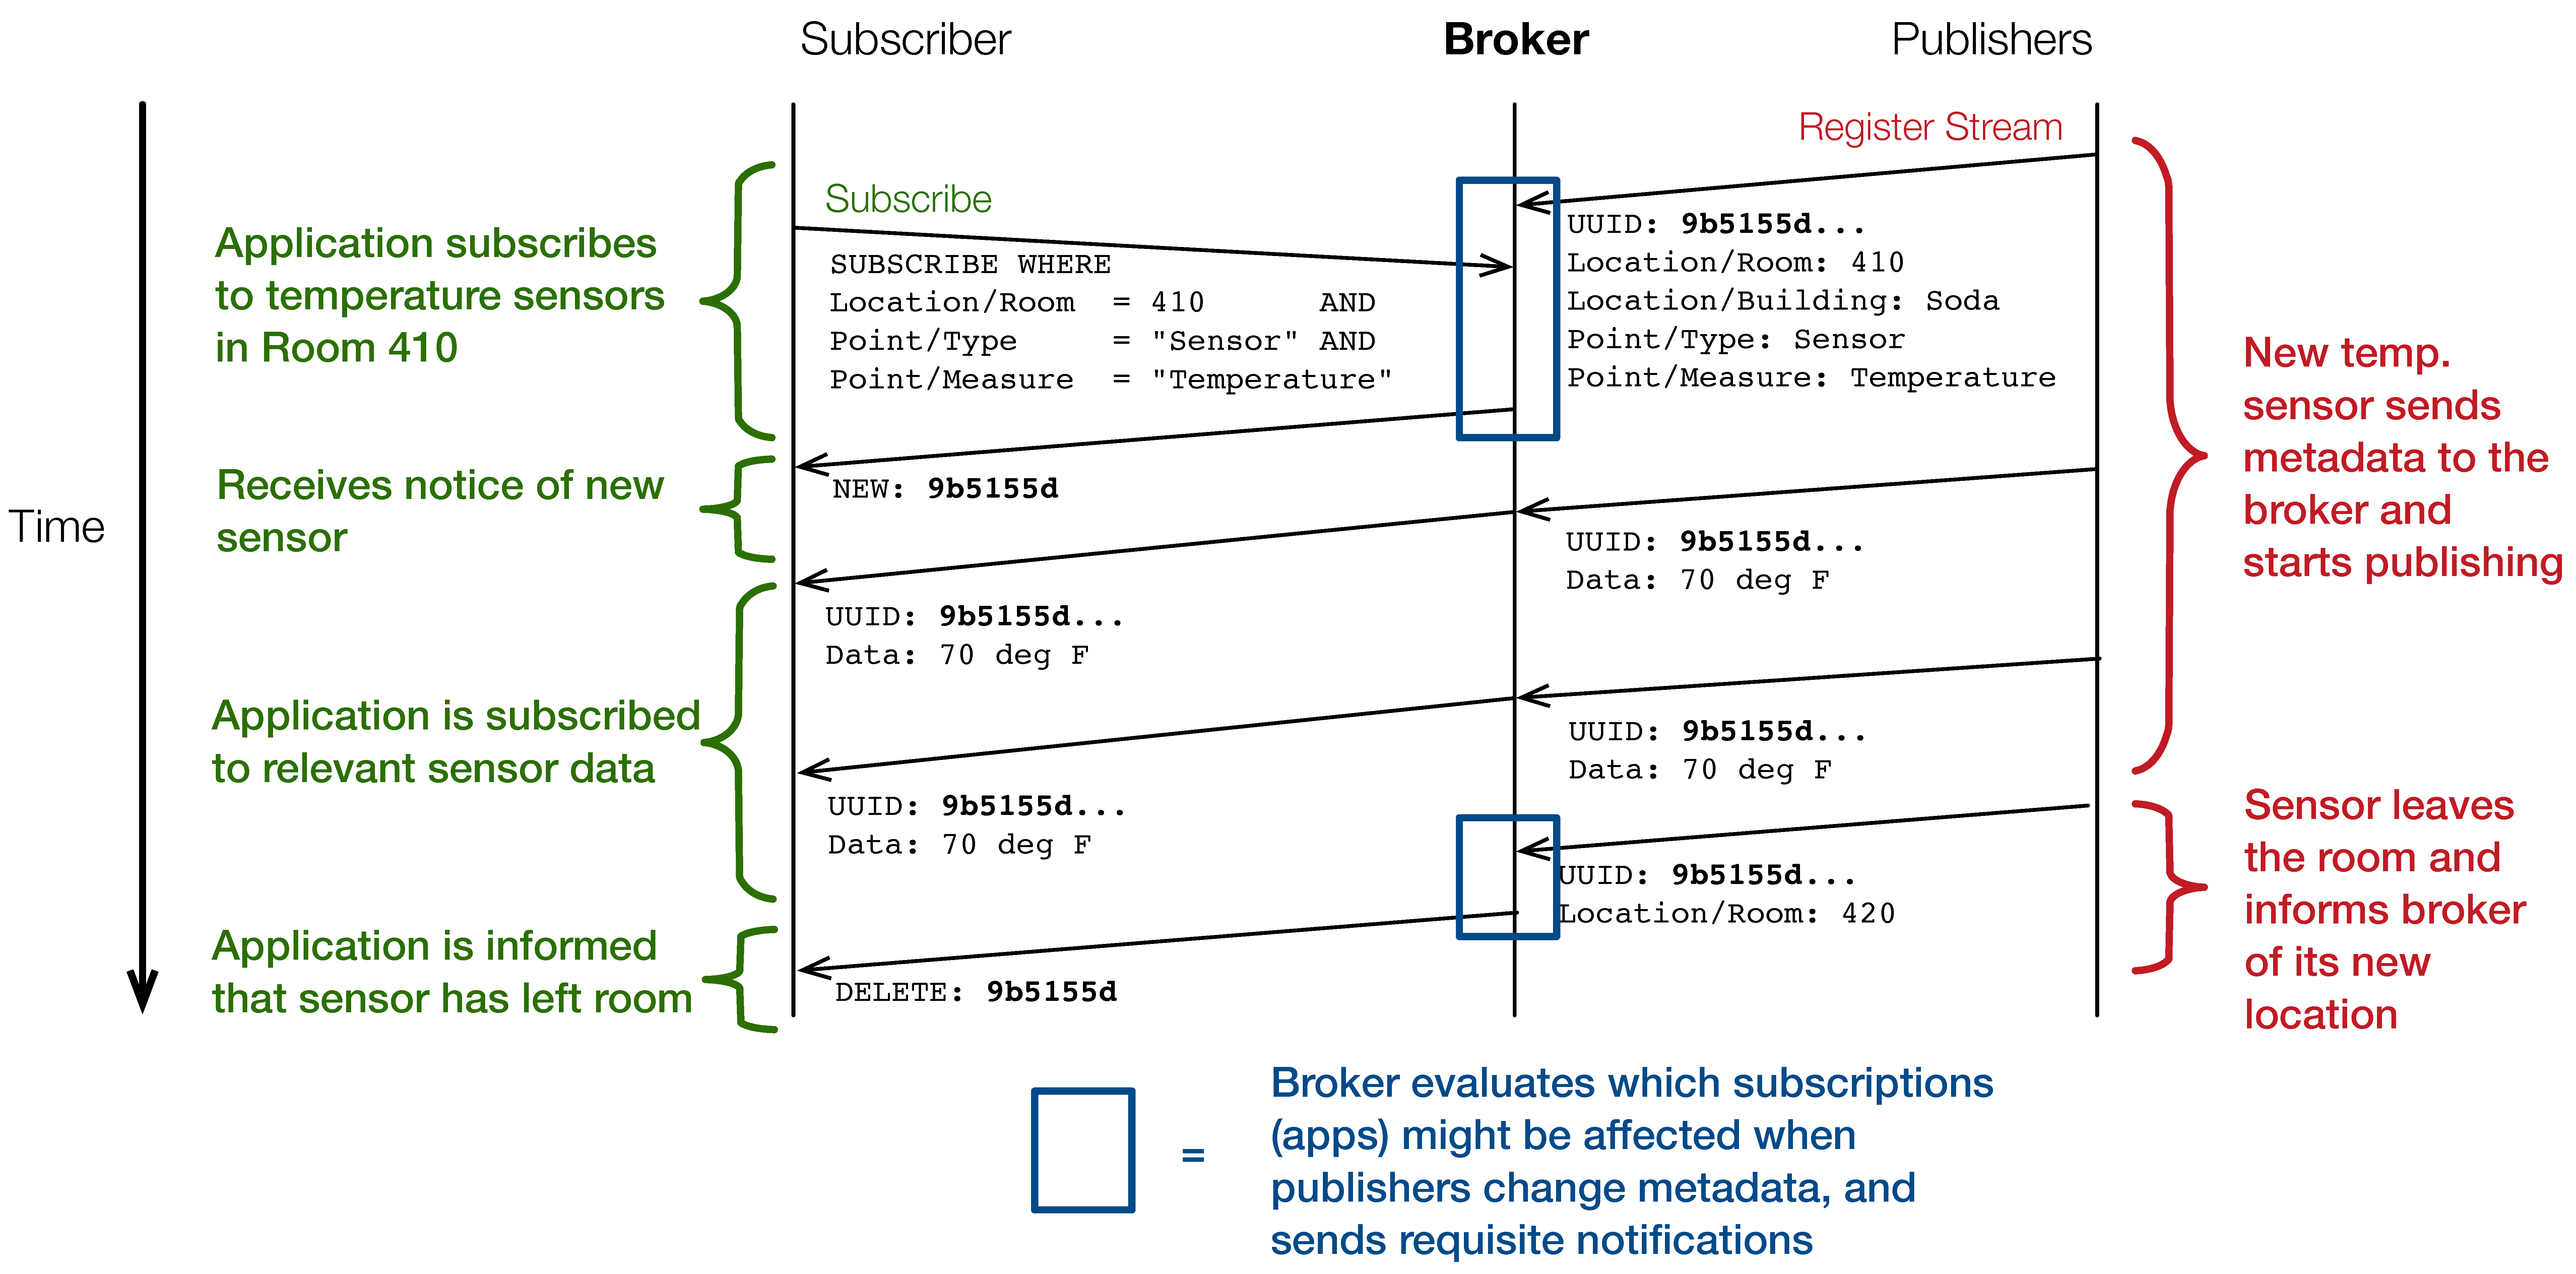
\includegraphics[width=.8\linewidth]{figs/messages.pdf}
\caption{The network traffic for a continuous query for discovering all temperature sensors in room 410 (ommitted
for brevity are additional constrains for building, units, etc). As new streams are registered, or their metadata
changes to no longer fit the discovery constraints, the client is updated in real-time.}
\label{fig:messages}
\end{figure*}


Queries are simple strings similar to the "where" clause of a SQL query. 
These predicates support basic operations on keys and values: equality, regex matching, existence, and combinations of these using \texttt{and}, \texttt{or} and \texttt{not}.
%Table~\ref{table:operations} contains the set of available operations over keys and values.

For example, a hypothetical daylighting application wants to adjust the brightness of lights corresponding to how much natural light is entering a room.
It subscribes to the output of all dimmable lights in room 410 as well as all illumination sensors.
There are two subscriptions:

\begin{minipage}{\linewidth}
\begin{sqlcode}
-- dimmable lights
Room = 410 AND System = "Lighting"
AND has Actuator/Brightness
-- illumination sensors
Room = 410 AND Point/Type = "Sensor"
AND Point/Measure = "Illumination"
\end{sqlcode}
\end{minipage}
\vspace{0.3cm}

Figure~\ref{fig:messages} illustrates a typical exchange of messsages.
First, a temperature sensor stream with UUID (starting with) \texttt{9b5155d} is registered as being in Room 410.
Then, an application enacts a subscription to all temperature sensors in 410 Soda.
The broker evaluates this query against its metadata store, and establishes forwarding paths for those streams.
The broker then informs the subscriber of the set of streams it is subscribed to.
As the sensor publishes, its messages are forwarded to the subscriber.
Finally, the sensor is moved to another room --- perhaps as part of a piece of smart clothing or furniture --- and informs the broker of the change in its metadata.
The broker sees that the \texttt{Location/Room} tag has changed, so it looks internally for all syndication queries that contain the \texttt{Location/Room} key.
The broker reevaluates each of these queries, informs the application of the change in the set of its subscribed streams, and then adjusts the forwarding paths.

\subsection{CQBS Broker Design}

Continuous queries are an extension of traditional request-response relational queries to capture changes in a query's result set over time.
All incoming queries are evaluated against the metadata database or returned from a cache.
After the initial results of the discovery query are returned, the broker will continue to deliver updates on the result set to the subscribed client.

The broker maintains several data structures that are updated on any metadata event -- such as registering streams, deleting streams or streams changing metadata -- to avoid needing to reevaluate all registered subscriptions on every single event.
The data structures provide fast lookup of all queries that involve a given metadata key, and store the mapping from a query to the set of the UUIDs for matched streams.

We decouple the metadata and query mechanism from the underlying database by implementing the query language using Go-yacc.
This grants the ability to inject functionality at intermediate levels of the parsing process.
For each submitted syndication query, the broker extracts the set of metadata keys to optimize the query reevaluation process, which involves two data structures.

The key-query table (the first data structure) maps metadata keys to the set of queries that involve them.
Queries are consistently hashed to avoid amplification of the lookup table by duplicate queries with reordered clause terms.
Any incoming metadata event will have its keys referenced against this lookup table, generating a set of queries that will need to be reevaluated after the incoming metadata changes are committed.
The second data structure, the query-UUID table, stores which streams have been resolved for each query.
It is updated whenever a query is evaluated, and simplifies identifying which streams have entered or left a result set for a given query upon a metadata event.

\subsection{Implementation}

The CQBS broker is implemented in Go~\cite{go}, a statically typed, garbage-collected language with language-level support for concurrency in the
form of multithreading as well as handling asynchronous operations.
The language contains several built-in concurrency primitives: goroutines (lightweight processes), channels (for message passing) and a \texttt{select} statement (which helps implement non-blocking operations).
For these reasons, the Go language is a natural fit for developing highly concurrent network systems.

Go channels, in both the buffered and unbuffered varieties, make relaying backpressure straightforward.
Using channels to convey incoming and outgoing data between pipelined components means that when a component is too loaded to respond to pending tasks, it simply does not dequeue new tasks from the incoming channel.
This forces upstream components to block in relaying their tasks to that component, and results in cascading backpressure extending to the client~\cite{welsh2001seda}.
It is important to note that this backpressure is only applied to publishers when they are sending faster than the broker can sustain, \emph{not} when a particular subscribed client is overloaded.

Having to manage queries against an underlying database during metadata changes introduces a number of blocking operations into the ``hot path'' of the broker.
Goroutines, combined with synchronization primitives such as \texttt{sync.WaitGroup}\footnote{\url{https://golang.org/pkg/sync/#WaitGroup}} from the Go standard library, are a natural way to dispatch multiple concurrent operations in parallel and wait for their completion.
Goroutines are scheduled by the Go runtime, and scale nicely over multiple cores.

The design and implementation of Go does pose several challenges for low-latency systems.
First among these is the garbage collector, which is non-generational and mark-and-sweep.
Concurrent garbage collection was introduced in Go 1.5, but heap allocations do noticeably contribute to increasing latency.
Because Go is garbage collected, a large number of heap allocations can incur high latencies during
operation.
Many protocol encoder/decoders in Go create many temporary objects, and Go's compile-time escape analysis unnecessarily promotes many stack allocations to heap allocations, as revealed
in \cite{goescape}.

Using typed formats such as MsgPack, CapnProto and Protobuf allows parsing code to ``plan-ahead'' for which types to use and how much space they will use.
JSON is particularly bad at this; because it is a character-based format, parsing it requires many intermediate buffers and lookaheads to determine the size and type of elements in a received message.
Using generated code for encoding/decoding can drastically reduce the number of allocations. We use the excellent \texttt{msgp} library\footnote{https://github.com/tinylib/msgp}, which reduced the allocations per message from roughly 20 to 3.

%Using the broker as an intermediary for all client communication means
%that clients need only implement a single application protocol while retaining
%the ability to ``talk'' to any other client by means of the broker. The broker
%handles all routing of messages, and its protocol plugins handle all necessary
%conversions to and from a client's established protocol. This also means that
%duty-cycled embedded clients can be discovered even if they are not active at
%the time of some inquiry; embedded clients can pull persisted data like
%actuation requests and updated discovery results from the broker upon waking.

%Continuous query-based syndication is made tractable by the coordination of the broker and query processor.
%The query processor keeps those bindings consistent with streams' changing metadata.

%The Giles broker reevalutes these syndication queries as the underlying streams change, ensuring that subscribed clients always have up-to-date information on the state of the system.

%%% Local Variables:
%%% mode: latex
%%% TeX-master: "paper.tex"
%%% End:
